\documentclass[10pt, a4paper,spanish]{article}
\usepackage[utf8]{inputenc}

\usepackage{lipsum} % Package to generate dummy text throughout this template
\usepackage{varwidth}
\usepackage{hyperref}
\usepackage{graphicx}
\graphicspath{ {images/} }

\usepackage[T1]{fontenc} % Use 8-bit encoding that has 256 glyphs
\usepackage{microtype} % Slightly tweak font spacing for aesthetics

\usepackage[hmarginratio=1:1,top=32mm,columnsep=20pt]{geometry} % Document margins
\usepackage[hang, small,labelfont=bf,up,textfont=it,up]{caption} % Custom captions under/above floats in tables or figures
\usepackage{booktabs} % Horizontal rules in tables
\usepackage{float} % Required for tables and figures in the multi-column environment - they need to be placed in specific locations with the [H] (e.g. \begin{table}[H])
\usepackage{hyperref} % For hyperlinks in the PDF

\usepackage{lettrine} % The lettrine is the first enlarged letter at the beginning of the text
\usepackage{paralist} % Used for the compactitem environment which makes bullet points with less space between them

\usepackage{abstract} % Allows abstract customization
\renewcommand{\abstractnamefont}{\normalfont\bfseries} % Set the "Abstract" text to bold
\renewcommand{\abstracttextfont}{\normalfont\small\itshape} % Set the abstract itself to small italic text

\usepackage{titlesec} % Allows customization of titles
\renewcommand\thesection{\Roman{section}} % Roman numerals for the sections
\renewcommand\thesubsection{\Roman{subsection}} % Roman numerals for subsections
\titleformat{\section}[block]{\large\scshape\centering}{\thesection.}{1em}{} % Change the look of the section titles
\titleformat{\subsection}[block]{\large}{\thesubsection.}{1em}{} % Change the look of the section titles
\usepackage{enumitem}

\usepackage{fancyhdr} % Headers and footers
\pagestyle{fancy} % All pages have headers and footers
\fancyhead{} % Blank out the default header
\fancyfoot{} % Blank out the default footer
\fancyhead[C]{ \today \ $\bullet$ PDSC $\bullet$ Tarea de Acortamiento} % Custom header text
\fancyfoot[RO,LE]{\thepage} % Custom footer text

%----------------------------------------------------------------------------------------
%	TITLE SECTION
%----------------------------------------------------------------------------------------

\title{\vspace{-15mm}\fontsize{24pt}{10pt}\selectfont\textbf{PDSC: Tarea de Acortamiento}} % Article title

\author{Sergio García Prado}
\date{\today}

%----------------------------------------------------------------------------------------

\begin{document}

	\maketitle % Insert title

	\thispagestyle{fancy} % All pages have headers and footers


%----------------------------------------------------------------------------------------
%	TEXT
%----------------------------------------------------------------------------------------

	\section{En el proyecto definido por las actividades indicadas calcular la duración total y el coste en condiciones normales. Si se precisara un acortamiento máximo de la duración del proyecto, ?`cuál sería la nueva duración y el coste resultante?. Realizar el acortamiento considerando un día cada vez.}

	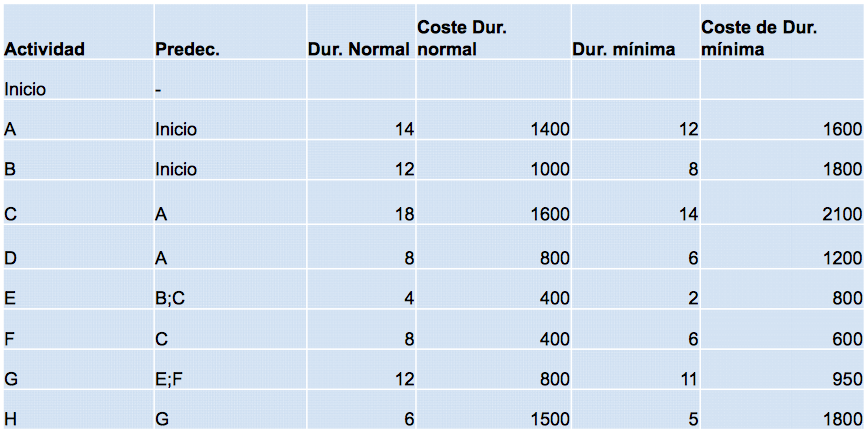
\includegraphics[width=\textwidth]{exercise-title}


	\paragraph{}
	La representación en forma de grafo de dicha red de actividades es la siguiente (en color rojo se indica el camino crítico):

	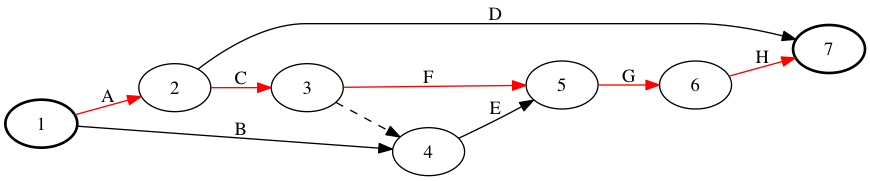
\includegraphics[width=\textwidth]{graph-2}

	\paragraph{}
	Por tanto, para obtener la duración del proyecto tan solo debemos realizar la suma de la duración de dichas tareas:
	\[
	T_A + T_C + T_F + T_G + T_H = 14 + 18 + 8 + 12 + 6 = 58
	\]
	Por lo cual sabemos que la duración normal del proyecto sería de \textbf{58 días}.

	\paragraph{}
	Para obtener el coste total del proyecto hay que realizar la suma de los costes de cada tarea:
	\[
	C_A + C_B + C_C + C_D + C_E + C_F + C_G + C_H = 1400 + 1000 + 1600 + 800 + 400 + 400 + 800 + 1500 = 7900
	\]

		Por lo cual sabemos que la el coste con una duración normal del proyecto sería de \textbf{7900 u.m.}.

	\paragraph{}
	Ahora supondremos que se quiere realizar un acortamiento día a día hasta llegar al máximo permitido. Para realizar este proceso se reducirá la tarea del camino crítico cuyo coste sea menor. Para realizar esta reducción se ha teniendo en cuenta la posibilidad de que el camino crítico pudiera variar(no ha sucedido).

	\paragraph{}
	Se ha conseguido por tanto reducir la duracción del proyecto en \textbf{10 días}, lo que fija la duración total del mismo en \textbf{48 días}. Para conseguir esto existe un incremento de \textbf{1350 u.m} en el coste, por lo cual el proyecto total tendría un nuevo coste de \textbf{9250 u.m.}.

	\paragraph{}
	En las siguientes tablas se muestra el proceso de acortamiento paso a paso:
	\break

	\noindent
	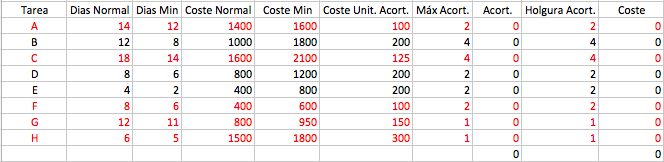
\includegraphics[width=\textwidth]{table-02}
	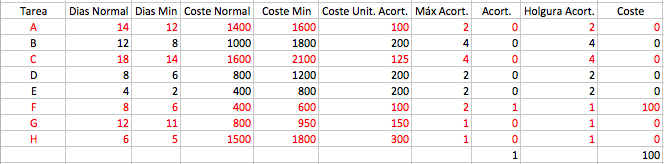
\includegraphics[width=\textwidth]{table-03}
	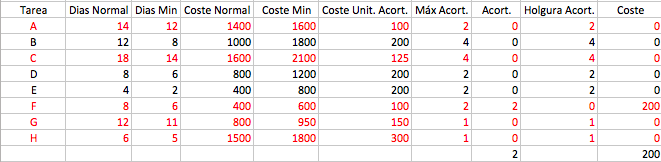
\includegraphics[width=\textwidth]{table-04}
	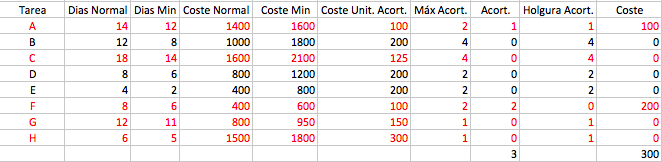
\includegraphics[width=\textwidth]{table-05}
	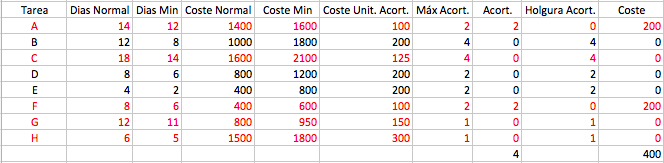
\includegraphics[width=\textwidth]{table-06}
	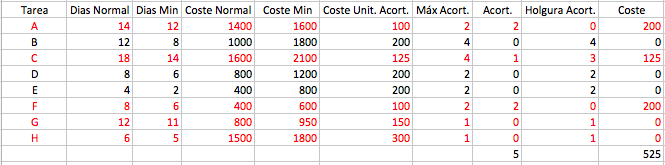
\includegraphics[width=\textwidth]{table-07}
	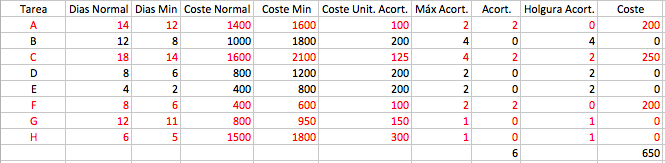
\includegraphics[width=\textwidth]{table-08}
	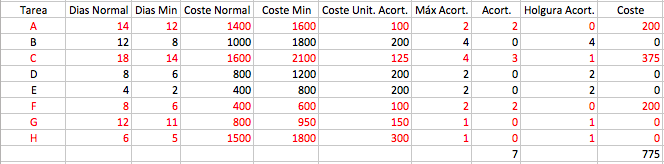
\includegraphics[width=\textwidth]{table-09}
	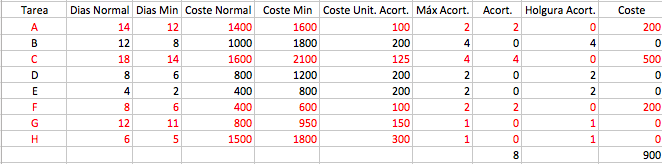
\includegraphics[width=\textwidth]{table-10}
	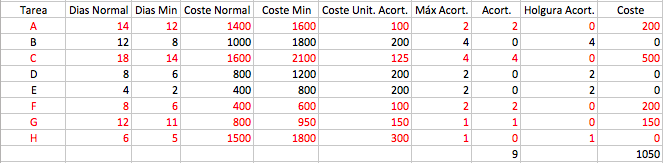
\includegraphics[width=\textwidth]{table-11}
	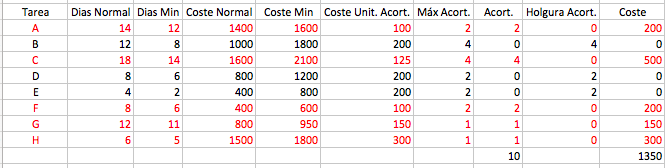
\includegraphics[width=\textwidth]{table-12}


\end{document}
